\section{Contexto e Motivação}

A perda de membros superiores representa um dos maiores desafios para a qualidade de vida de indivíduos acometidos por amputações traumáticas, congênitas ou decorrentes de doenças como diabetes e doenças vasculares periféricas. No Brasil, segundo dados do Sistema de Informações Hospitalares do SUS (SIH/SUS), foram realizados 49.165 procedimentos de amputação em 2011, sendo as causas externas (33,1\%), doenças infecciosas e parasitárias (17,9\%) e doenças do aparelho circulatório (16,1\%) as etiologias mais frequentes. Apesar de as amputações de membros inferiores corresponderem a aproximadamente 85\% de todos os casos, as amputações de membros superiores impõem impacto funcional severo, comprometendo diretamente a autonomia e a capacidade de realização das atividades de vida diária do indivíduo. \cite{Diretrizes}
\begin{figure}[htbp]
    \centering
    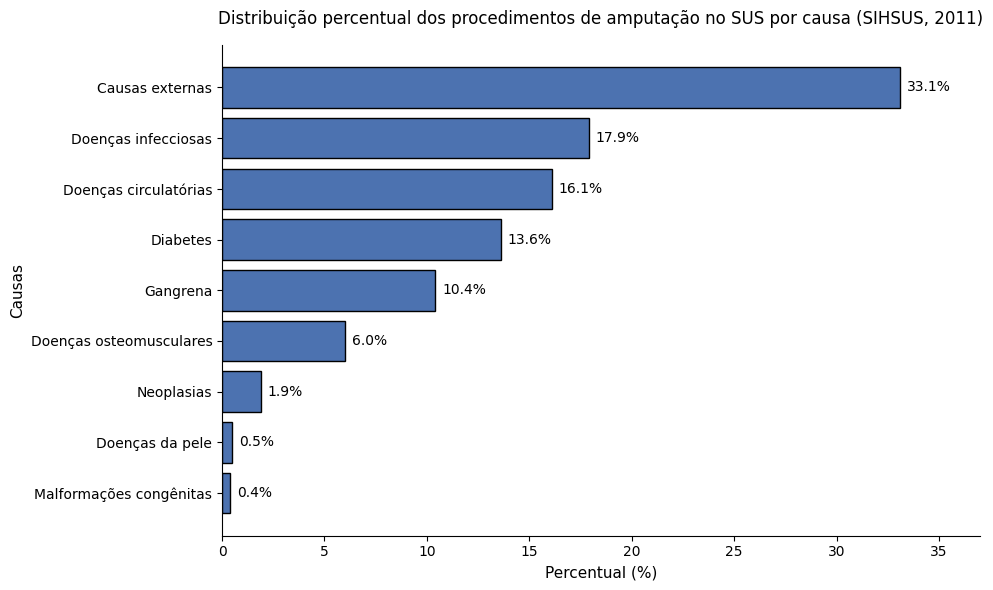
\includegraphics[width=0.8\textwidth]{1_introducao/assets/frequencia_amputacao.png}
    \caption{Distribuição percentual dos procedimentos de amputação no SUS por causa \cite{Diretrizes}.}
    \label{fig:amputacoes}
\end{figure}

Neste cenário, as próteses robóticas controladas por sinais biológicos emergem como uma alternativa promissora.